%%%%%%%%%%%%%%%%%%%%%%%%%%%%%%%%%%%%%%%%%%

\chapter{Demonstration of simultaneous spin analyzer}\label{chap:ssa_2020}

%%%%%%%%%%%%%%%%%%%%%%%%%%%%%%%%%%%%%%%%%%

Measurements took place in 2020. Initial version of \acrshort{ssa} was tested. All measurements are flow through measurements from source to spin analyzer

\begin{figure}
    \centering
    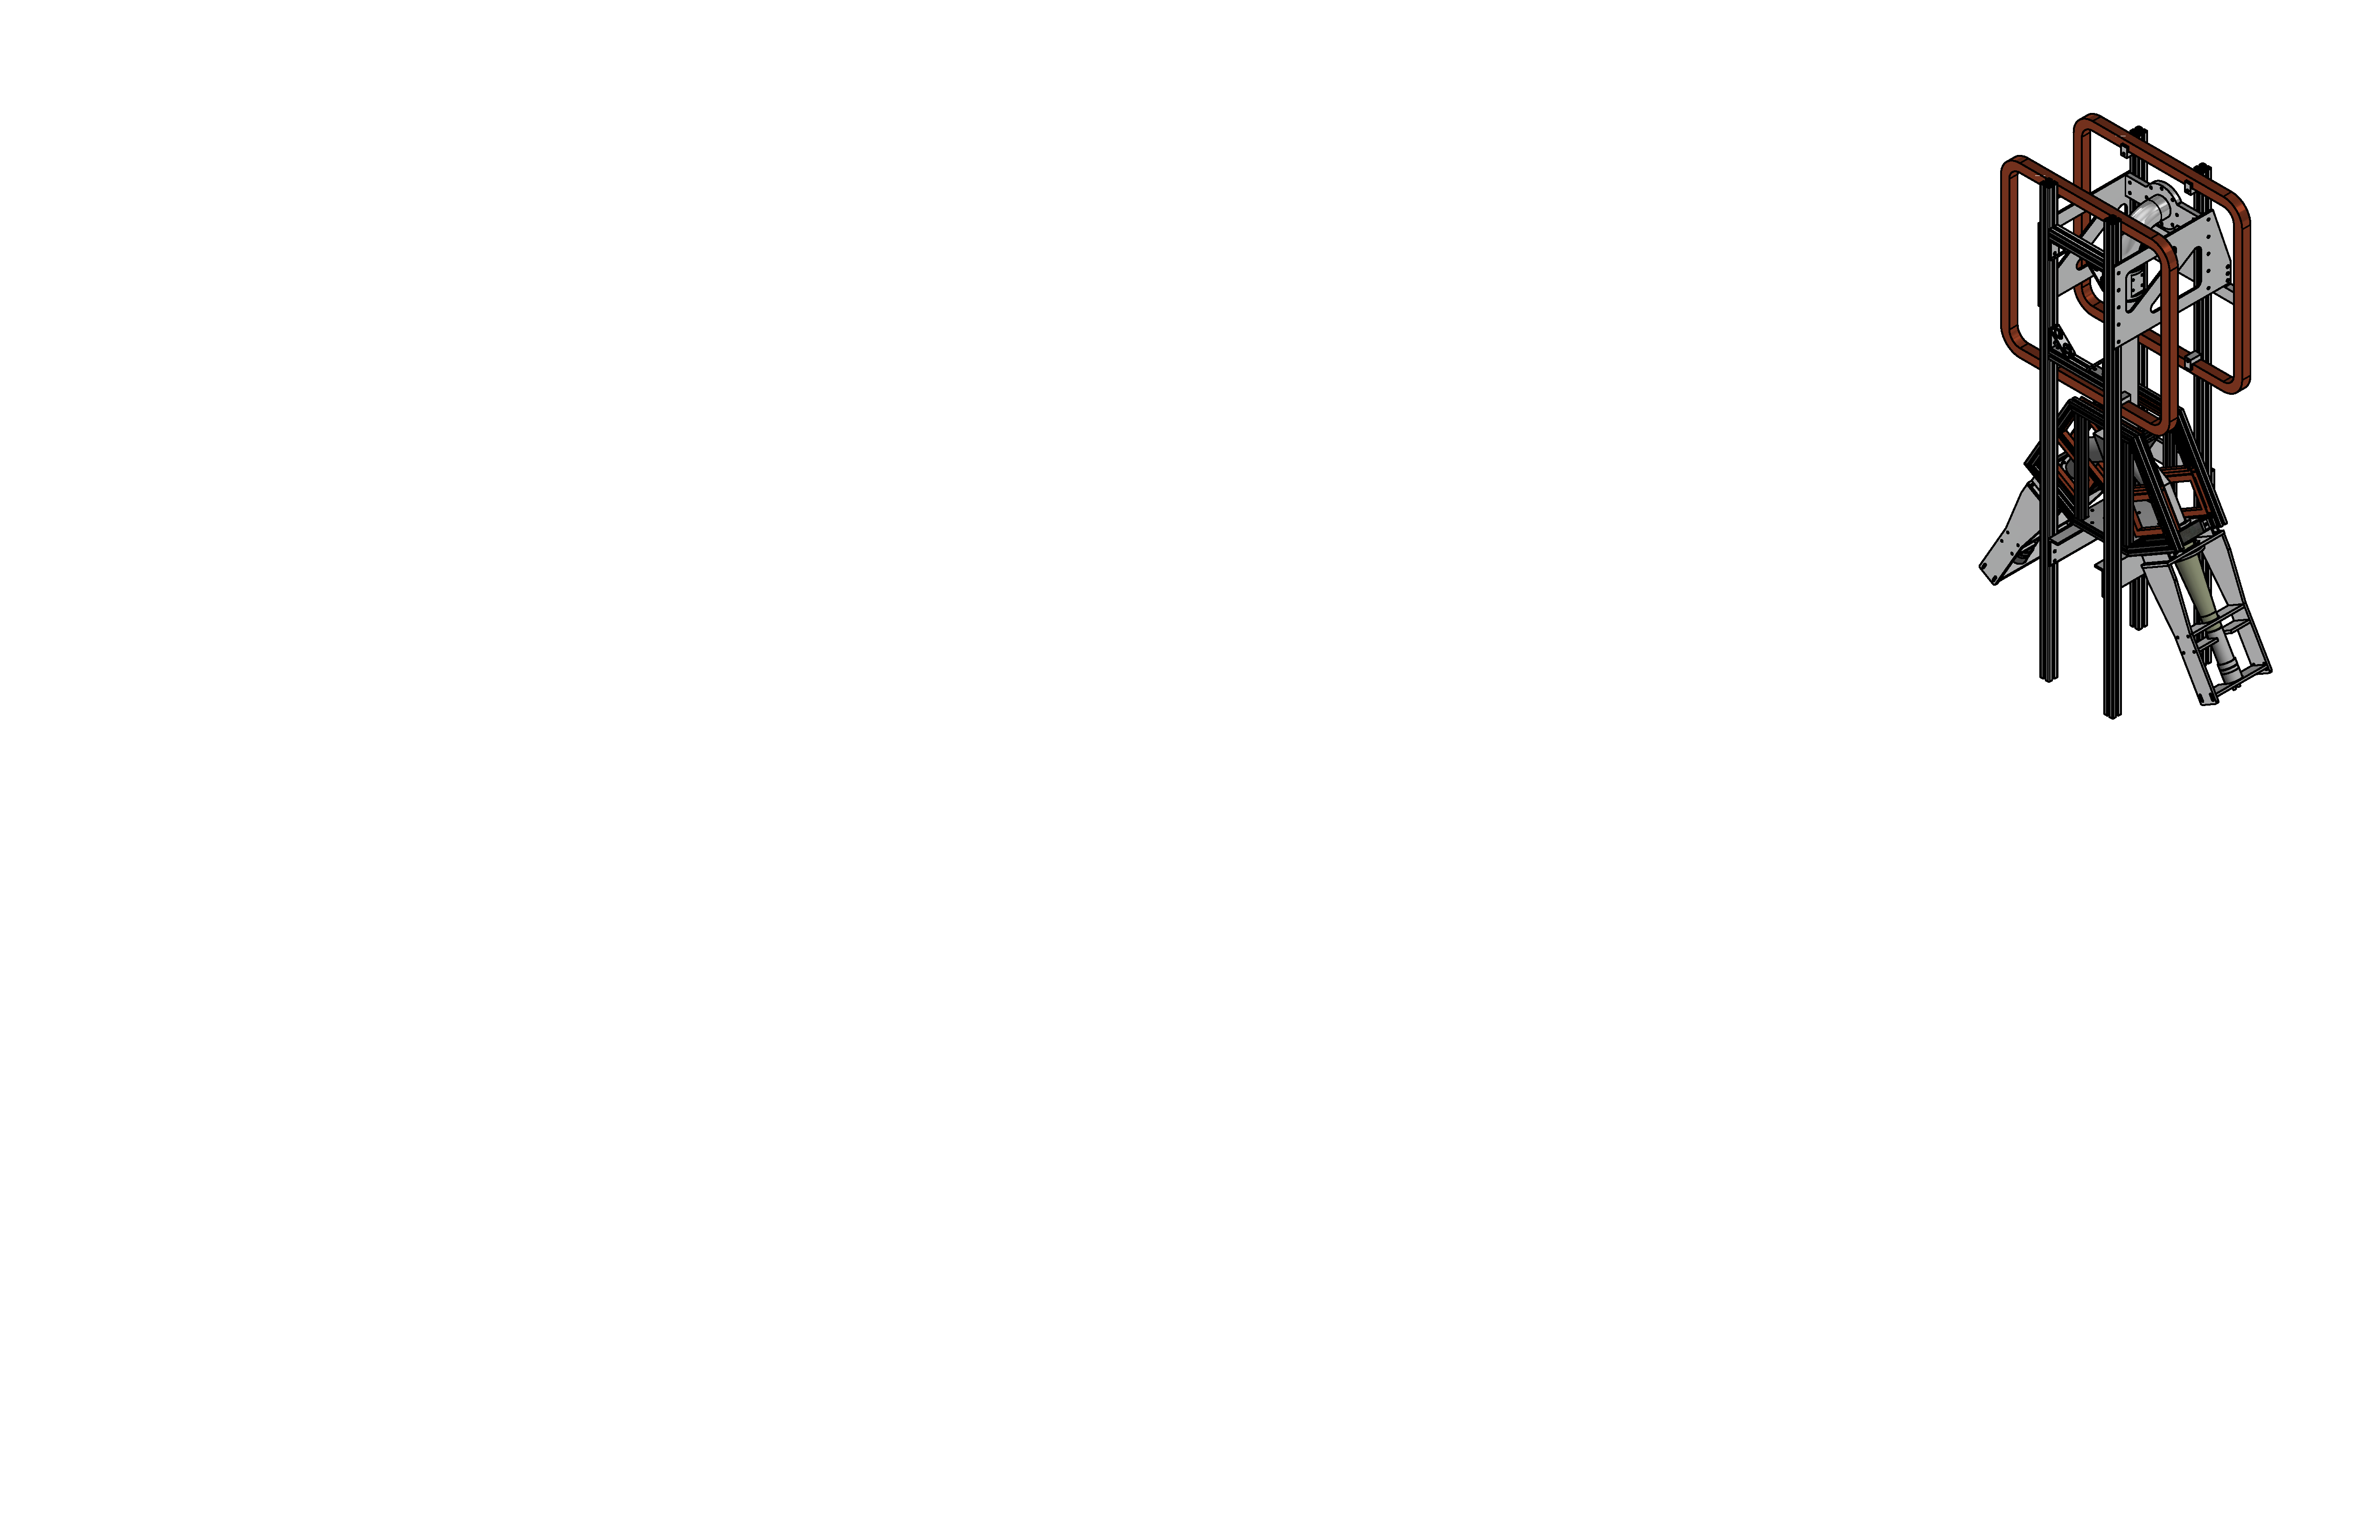
\includegraphics[height=3.1in]{figures/ssa_schematic_colorized.pdf}
    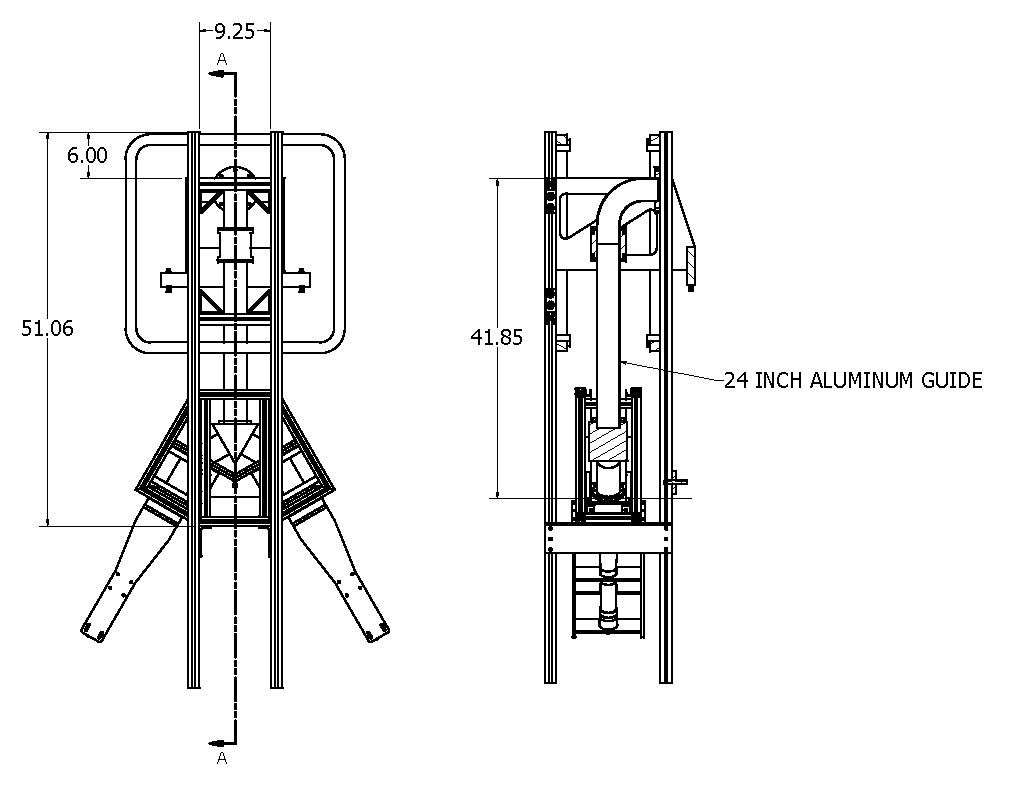
\includegraphics[height=3.5in]{figures/ssa_schematics.pdf}
    \caption
    {Schematics for first iteration of simultaneous spin analyzer, mounting frame, and associated transport coils. Courtesy of Mark Luxnat.}
    \label{fig:ssa_schematic}
\end{figure}

%%%%%%%%%%%%%%%%%%%%%%%%%%%%%%%%%%%%%%%%%%

\section{Description of apparatus}

%%%%%%%%%%%%%%%%%%%%%%%%%%%%%%%%%%%%%%%%%%

Same polarizer, \BZnS scintillator , iron yoke design. Mounted on a free switcher port. Other port had the single arm. 

%%%%%%%%%%%%%%%%%%%%%%%%%%%%%%%%%%%%%%%%%%

\section{Measurements}

%%%%%%%%%%%%%%%%%%%%%%%%%%%%%%%%%%%%%%%%%%

To limit the impact on the UCN source, used these beam parameters: 

\begin{small}
\begin{verbatim}
-------------------------------------------------
beam parameters for the nEDM test measurements
capture H-Gx: 77%
countdown: 1---> 8
pattern width: 327
9 pulses per burst
4.975 s between bursts
---------------------------------------------------
Average current = 1 micro-A

This should lower the current by a factor of 10.

\end{verbatim}
\end{small}

Beam continuously on. North gate valve toggled on and off every 30 seconds to allow detectors to drain (and avoid cross talk influencing the next step). Counting integration period is the middle 20 seconds of the 30 second NGV open stage to avoid the spike of neutrons when gate opens.



\begin{figure}
    \centering
    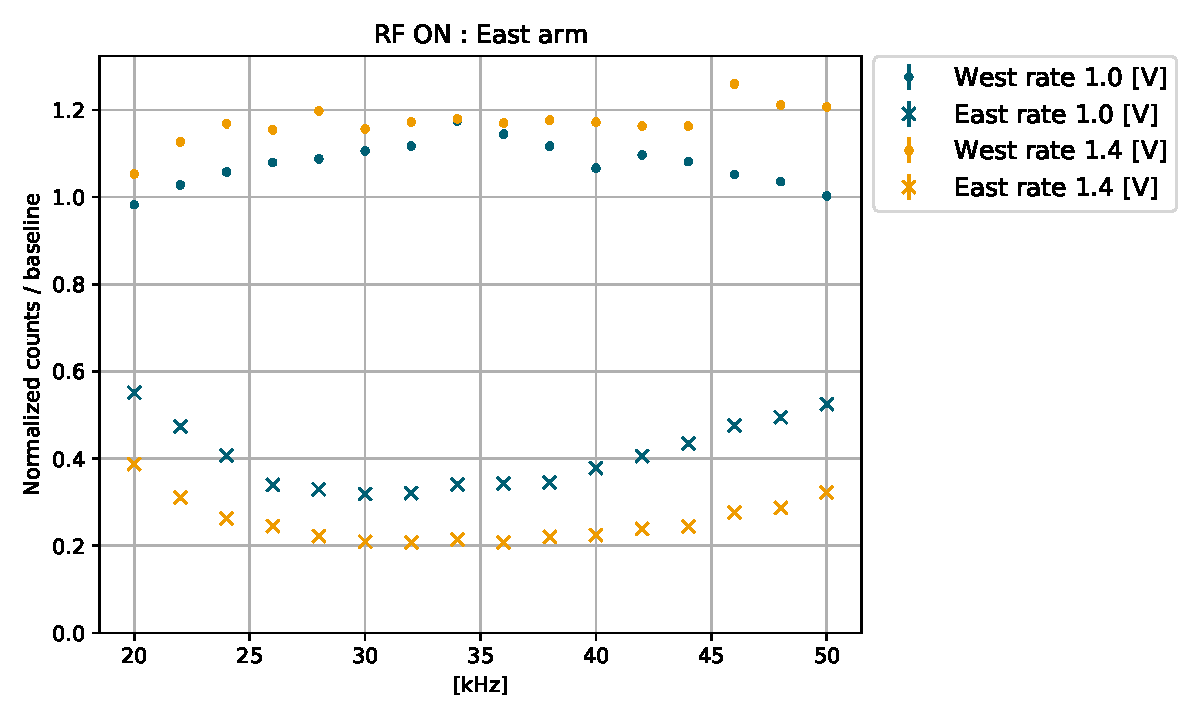
\includegraphics[width=0.7\textwidth]{figures/RF_ON_East_arm.pdf}
    \caption
    [Flow through measurement of UCN from the source to the simultaneous spin analyzer, with the RF spin flipper on the ``East'' arm energized.]
    {Flow through measurement of UCN from the source to the simultaneous spin analyzer, with the RF spin flipper on the ``East'' arm energized. Measurements for various peak-to-peak amplitudes on the RF function generator are shown. Normalized detector counts on the $y$-axis are depicted as a fraction of the respective detector's baseline count rate with the RF spin flipper off. Error bars are smaller than the markers}
    \label{fig:Fall2020_SSA_RF_east}
% \end{figure}
    \vspace{\baselineskip}
% \begin{figure}
    \centering
    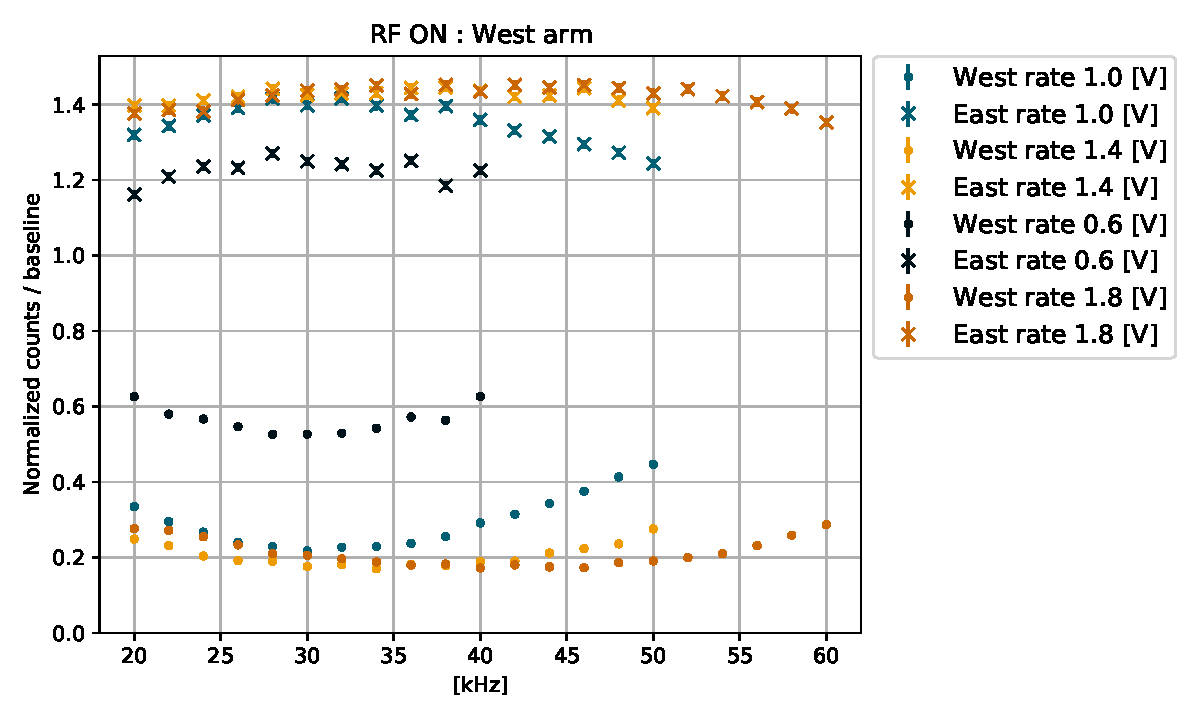
\includegraphics[width=0.7\textwidth]{figures/RF_ON_West_arm.pdf}
    \caption
    [Flow through measurement of UCN from the source to the simultaneous spin analyzer, with the RF spin flipper on the ``West'' arm energized.]
    {Flow through measurement of UCN from the source to the simultaneous spin analyzer, with the RF spin flipper on the ``West'' arm energized. Error bars are smaller than the markers.}\label{fig:Fall2020_SSA_RF_west}
\end{figure}

\begin{figure}
\centering
%subfigure width gets "multiplied" by includegraphics width
\begin{subfigure}{.5\textwidth} 
  \centering
  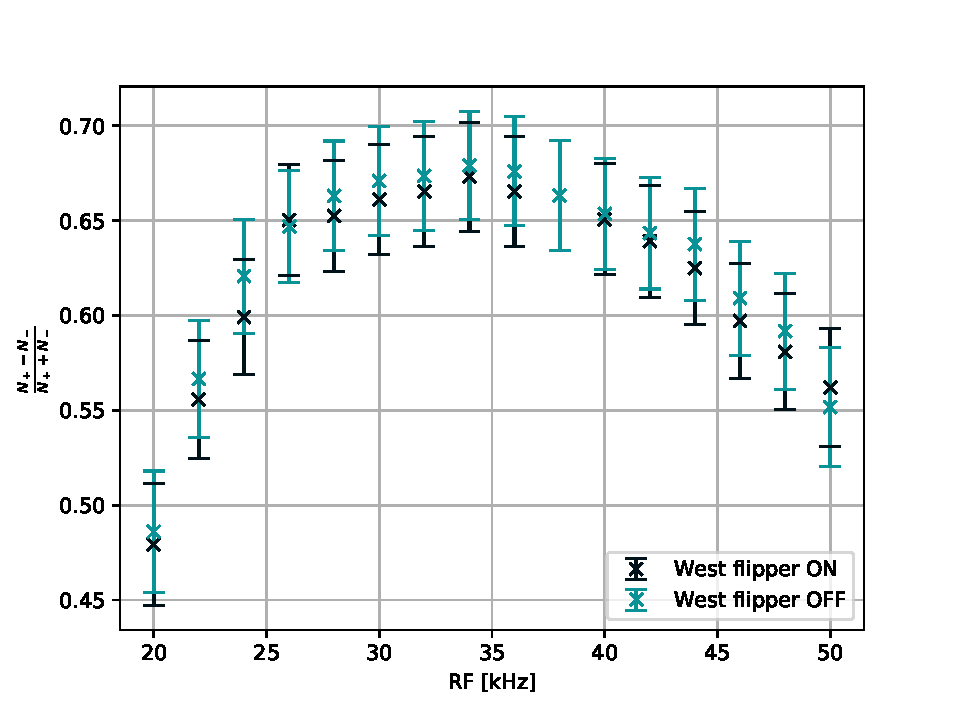
\includegraphics[width=\textwidth]{figures/SSA_east_arm_no_west_foil.pdf}
  \caption{East arm asymmetry, no foil on West arm }\label{subfig:SSA_east_arm_no_west_foil}
\end{subfigure}%DO NOT REMOVE THIS '%'
\begin{subfigure}{.5\textwidth}
  \centering
  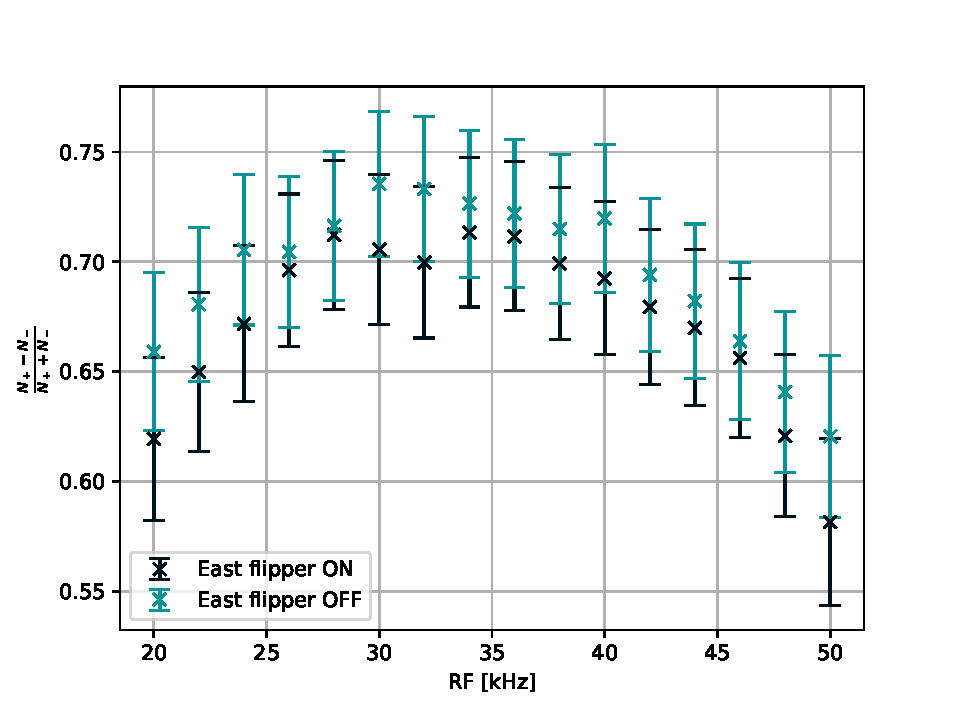
\includegraphics[width=\textwidth]{figures/SSA_west_arm_no_west_foil.pdf}
  \caption{West arm asymmetry, no foil on East arm}\label{subfig:SSA_west_arm_no_west_foil}
\end{subfigure}
\caption
    {Spin symmetry measurement in one arm of the simultaneous spin analyzer, with the polarizing foil on the opposite arm removed. ($V_\text{pp}=\qty{1.4}{V}$)}
\label{fig:SSA_asym_one_foil_out}
\end{figure}

%%%%%%%%%%%%%%%%%%%%%%%%%%%%%%%%%%%%%%%%%%

\section{Discussion}

%%%%%%%%%%%%%%%%%%%%%%%%%%%%%%%%%%%%%%%%%%

Observe that as neutrons get rejected from one arm, the other arm sees increased counts 

Flow through measurement of single arm for comparison in Fig.~\ref{fig:spin_flipper_efficiency}. (Minimum at 0.12. Asymmetry = 0.8). Fig.~\ref{fig:Fall2020_SSA_RF_east}, for RF ON, Amp=1.4 V at 34 kHz, minimum at 0.21, Asymmetry = 0.65. Fig.~\ref{fig:Fall2020_SSA_RF_east}, for RF ON, Amp=1.4 V at 34 kHz, minimum at 0.17, Asymmetry = 0.69.

If gradient is small resonance is narrow, because B0 must match B1 on RF for adiabaticity

Check chances of a rejected on one arm being depolarized and allowed through the other arm. Fig.~\ref{fig:SSA_asym_one_foil_out}. Asymmetry at 34 kHz East is 0.68. At West is 0.73, not particularly meaningful.

Wound RF coils with higher coil count and removed aluminum sleeve which might attenuate things (outer aluminum housing anyway).

Increased guide drop with NiP coated segment. For comparison, beneath the elbow, the single arm channel has a drop of \qty{39}{in} to the iron yoke.

New power supply with higher amplitude. keithley 6517b

PMTs changed out for SiPMs for a better vacuum seal and to avoid potential complications of PMTs under a large magnetic field

Silicon Photomultiplier(SiPM) 4-Side Scaleable Arrays. Array C Series